\section{\texorpdfstring{UViT-H/DC-AE:
center\_\allowbreak{}crop\_\allowbreak{}area50}{UViT-H/DC-AE: }}\label{record-docs-watermarking-qualitative-image-dcae-center-crop-area50-md-uvit-hdc-ae-center_crop_area50}

This reconstructs the documented JPEG-quality-50 or native center-crop
operation from the saved original PNG for display. Captions use the
originally recorded detector scores and transformed-calibration
threshold. Paired quality was not measured for these legacy output
transformations.

Eight pairs use fixed original indices 0, 64, 128, 192, 256, 320, 384
and 448. No detection or visual-quality filtering is applied.

\begin{recordfigure}
\centering
\pandocbounded{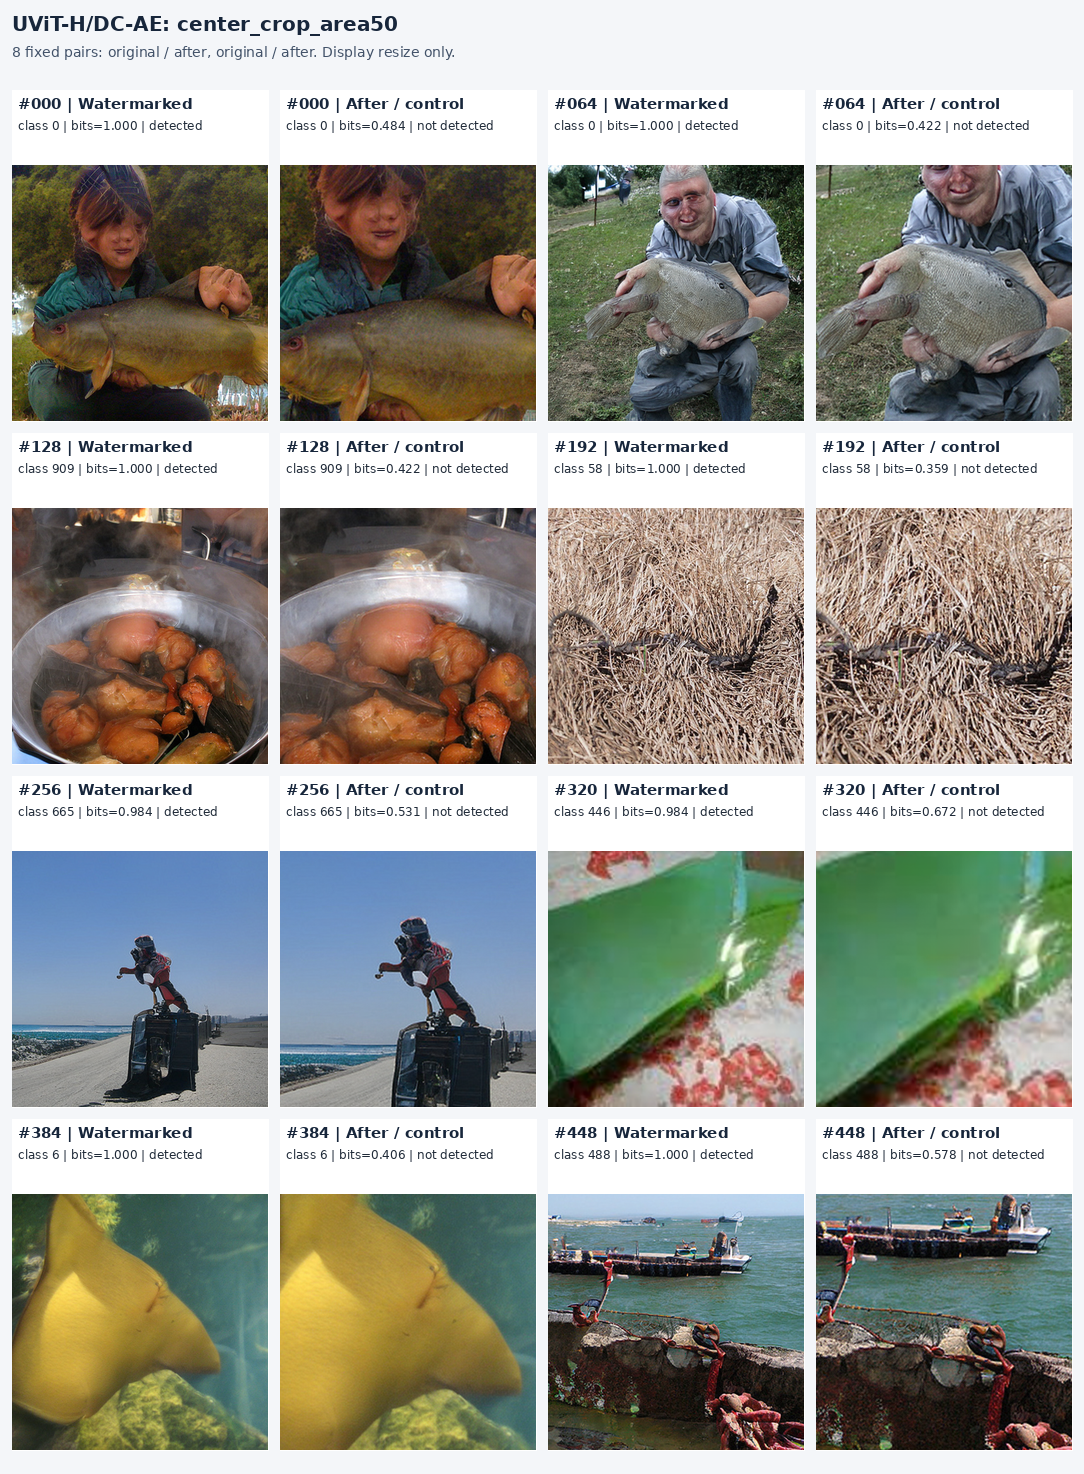
\includegraphics[keepaspectratio,alt={Eight original/after image pairs}]{figures/image-dcae-center_crop_area50.png}}
\caption{Eight original/after image pairs}
\end{recordfigure}

The lossless figure contains 16 panels. Each panel is displayed at 256
pixels; metrics use original native-resolution PNGs. Labels report each
output's detector result, not guaranteed removal.

{\scriptsize\setlength{\tabcolsep}{3pt}\def\LTcaptype{none} % do not increment counter
\begin{longtable}[]{@{}
  >{\raggedright\arraybackslash}p{(\linewidth - 10\tabcolsep) * \real{0.1667}}
  >{\raggedright\arraybackslash}p{(\linewidth - 10\tabcolsep) * \real{0.1667}}
  >{\raggedright\arraybackslash}p{(\linewidth - 10\tabcolsep) * \real{0.1667}}
  >{\raggedright\arraybackslash}p{(\linewidth - 10\tabcolsep) * \real{0.1667}}
  >{\raggedright\arraybackslash}p{(\linewidth - 10\tabcolsep) * \real{0.1667}}
  >{\raggedright\arraybackslash}p{(\linewidth - 10\tabcolsep) * \real{0.1667}}@{}}
\toprule\noalign{}
\begin{minipage}[b]{\linewidth}\raggedright
Index
\end{minipage} & \begin{minipage}[b]{\linewidth}\raggedright
Class
\end{minipage} & \begin{minipage}[b]{\linewidth}\raggedright
Before
\end{minipage} & \begin{minipage}[b]{\linewidth}\raggedright
After
\end{minipage} & \begin{minipage}[b]{\linewidth}\raggedright
LPIPS
\end{minipage} & \begin{minipage}[b]{\linewidth}\raggedright
Class CLIP
\end{minipage} \\
\midrule\noalign{}
\endhead
\bottomrule\noalign{}
\endlastfoot
0 & 0 & class 0 \textbar{} bits=1.000 \textbar{} detected & class 0
\textbar{} bits=0.484 \textbar{} not detected & not measured & not
measured \\
64 & 0 & class 0 \textbar{} bits=1.000 \textbar{} detected & class 0
\textbar{} bits=0.422 \textbar{} not detected & not measured & not
measured \\
128 & 909 & class 909 \textbar{} bits=1.000 \textbar{} detected & class
909 \textbar{} bits=0.422 \textbar{} not detected & not measured & not
measured \\
192 & 58 & class 58 \textbar{} bits=1.000 \textbar{} detected & class 58
\textbar{} bits=0.359 \textbar{} not detected & not measured & not
measured \\
256 & 665 & class 665 \textbar{} bits=0.984 \textbar{} detected & class
665 \textbar{} bits=0.531 \textbar{} not detected & not measured & not
measured \\
320 & 446 & class 446 \textbar{} bits=0.984 \textbar{} detected & class
446 \textbar{} bits=0.672 \textbar{} not detected & not measured & not
measured \\
384 & 6 & class 6 \textbar{} bits=1.000 \textbar{} detected & class 6
\textbar{} bits=0.406 \textbar{} not detected & not measured & not
measured \\
448 & 488 & class 488 \textbar{} bits=1.000 \textbar{} detected & class
488 \textbar{} bits=0.578 \textbar{} not detected & not measured & not
measured \\
\end{longtable}
}

\href{records/docs/watermarking/images.tex}{Image metrics} \textbar{}
\href{../docs/watermarking/README.md}{Report overview}
